\documentclass[12pt,letterpaper]{article}\usepackage[]{graphicx}\usepackage[]{color}
%% maxwidth is the original width if it is less than linewidth
%% otherwise use linewidth (to make sure the graphics do not exceed the margin)
\makeatletter
\def\maxwidth{ %
  \ifdim\Gin@nat@width>\linewidth
    \linewidth
  \else
    \Gin@nat@width
  \fi
}
\makeatother

\definecolor{fgcolor}{rgb}{0.345, 0.345, 0.345}
\newcommand{\hlnum}[1]{\textcolor[rgb]{0.686,0.059,0.569}{#1}}%
\newcommand{\hlstr}[1]{\textcolor[rgb]{0.192,0.494,0.8}{#1}}%
\newcommand{\hlcom}[1]{\textcolor[rgb]{0.678,0.584,0.686}{\textit{#1}}}%
\newcommand{\hlopt}[1]{\textcolor[rgb]{0,0,0}{#1}}%
\newcommand{\hlstd}[1]{\textcolor[rgb]{0.345,0.345,0.345}{#1}}%
\newcommand{\hlkwa}[1]{\textcolor[rgb]{0.161,0.373,0.58}{\textbf{#1}}}%
\newcommand{\hlkwb}[1]{\textcolor[rgb]{0.69,0.353,0.396}{#1}}%
\newcommand{\hlkwc}[1]{\textcolor[rgb]{0.333,0.667,0.333}{#1}}%
\newcommand{\hlkwd}[1]{\textcolor[rgb]{0.737,0.353,0.396}{\textbf{#1}}}%
\let\hlipl\hlkwb

\usepackage{framed}
\makeatletter
\newenvironment{kframe}{%
 \def\at@end@of@kframe{}%
 \ifinner\ifhmode%
  \def\at@end@of@kframe{\end{minipage}}%
  \begin{minipage}{\columnwidth}%
 \fi\fi%
 \def\FrameCommand##1{\hskip\@totalleftmargin \hskip-\fboxsep
 \colorbox{shadecolor}{##1}\hskip-\fboxsep
     % There is no \\@totalrightmargin, so:
     \hskip-\linewidth \hskip-\@totalleftmargin \hskip\columnwidth}%
 \MakeFramed {\advance\hsize-\width
   \@totalleftmargin\z@ \linewidth\hsize
   \@setminipage}}%
 {\par\unskip\endMakeFramed%
 \at@end@of@kframe}
\makeatother

\definecolor{shadecolor}{rgb}{.97, .97, .97}
\definecolor{messagecolor}{rgb}{0, 0, 0}
\definecolor{warningcolor}{rgb}{1, 0, 1}
\definecolor{errorcolor}{rgb}{1, 0, 0}
\newenvironment{knitrout}{}{} % an empty environment to be redefined in TeX

\usepackage{alltt}

\usepackage{amsmath}
\usepackage{bm} % for bold math symbols
\usepackage{booktabs} % better tables
\usepackage[left=.4in,right=.2in,top=.4in,bottom=.2in]{geometry} % margins
\usepackage{caption} % for subfigures
\usepackage[T1]{fontenc} % see http://goo.gl/KXXek
\usepackage{graphicx} % obviously for graphics
\usepackage{lscape}
\usepackage{listings} % source code
\usepackage{latexsym} % MBE template for some fonts
\usepackage{mathtools} % an extension to amsmath to fix bugs
\usepackage{multirow} % column cells that span multiple rows
\usepackage{natbib} % nicer references
\usepackage{paralist} % inline lists
\usepackage[section]{placeins} % keep figures and table inside section
\usepackage{setspace} % for line spacing
\usepackage{subfig} % for subfigures
%\usepackage{subcaption} % for subfigures (can't be used with subfig)
%\usepackage{tikz}
%\usepackage{tikz-qtree}
%\usetikzlibrary{arrows}
\IfFileExists{upquote.sty}{\usepackage{upquote}}{}
\begin{document}



\begin{itemize}
\item Simulation under the null for branch-site model A
\item Symmetric, 8-taxon tree with one foreground branch \\
  The total tree length is 3.\\
  tree: (((A\#1:0.214286,B:0.214286):0.214286,(C:0.214286,D:0.214286):0.214286):0.214286,((E:0.214286,F:0.214286):0.214286,(G:0.214286,H:0.214286):0.214286):0.214286);
\item $\kappa=2.0$ $p_0=0.7$ $p_{1}=0.2$ $\omega_0=0.3$
\end{itemize}

\begin{knitrout}
\definecolor{shadecolor}{rgb}{0.969, 0.969, 0.969}\color{fgcolor}

{\centering 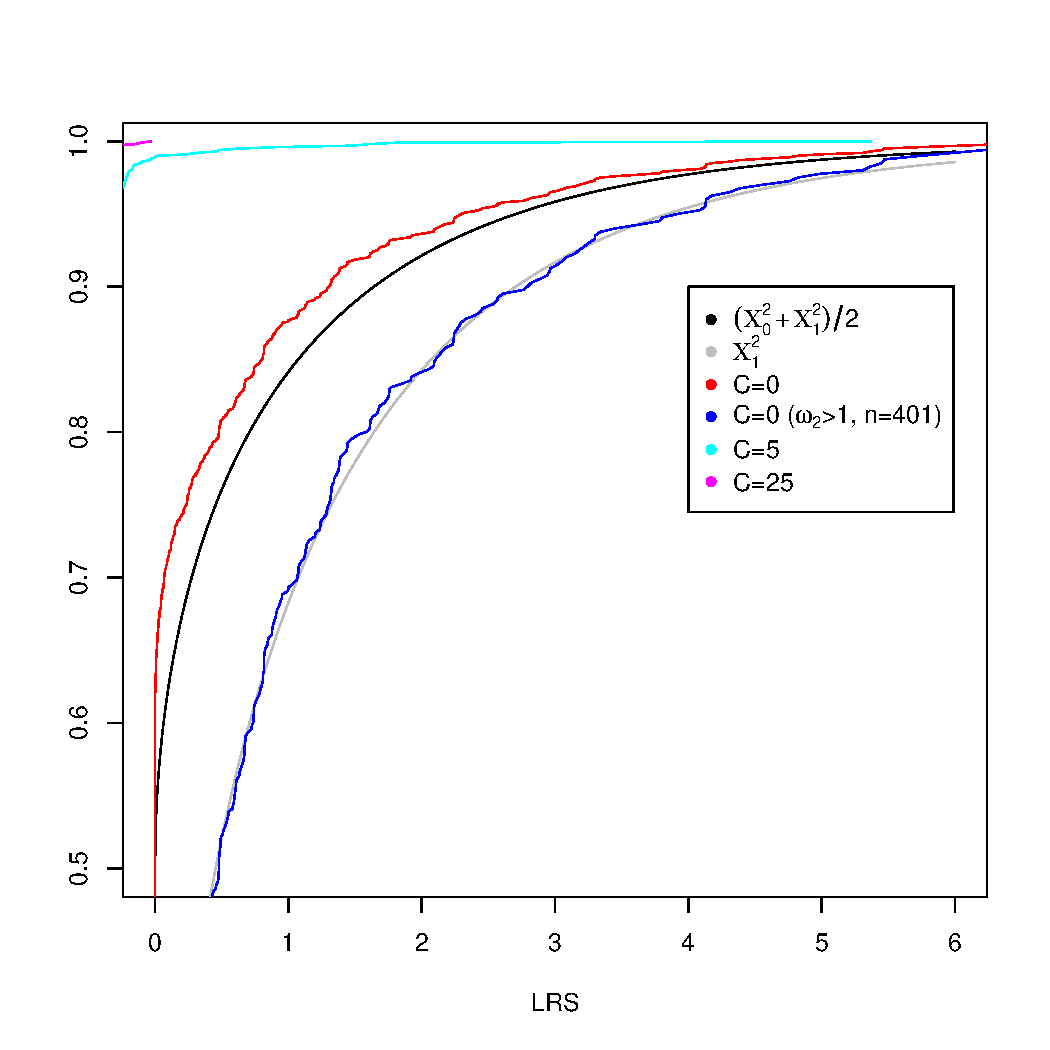
\includegraphics[width=\maxwidth]{figures/data-1} 
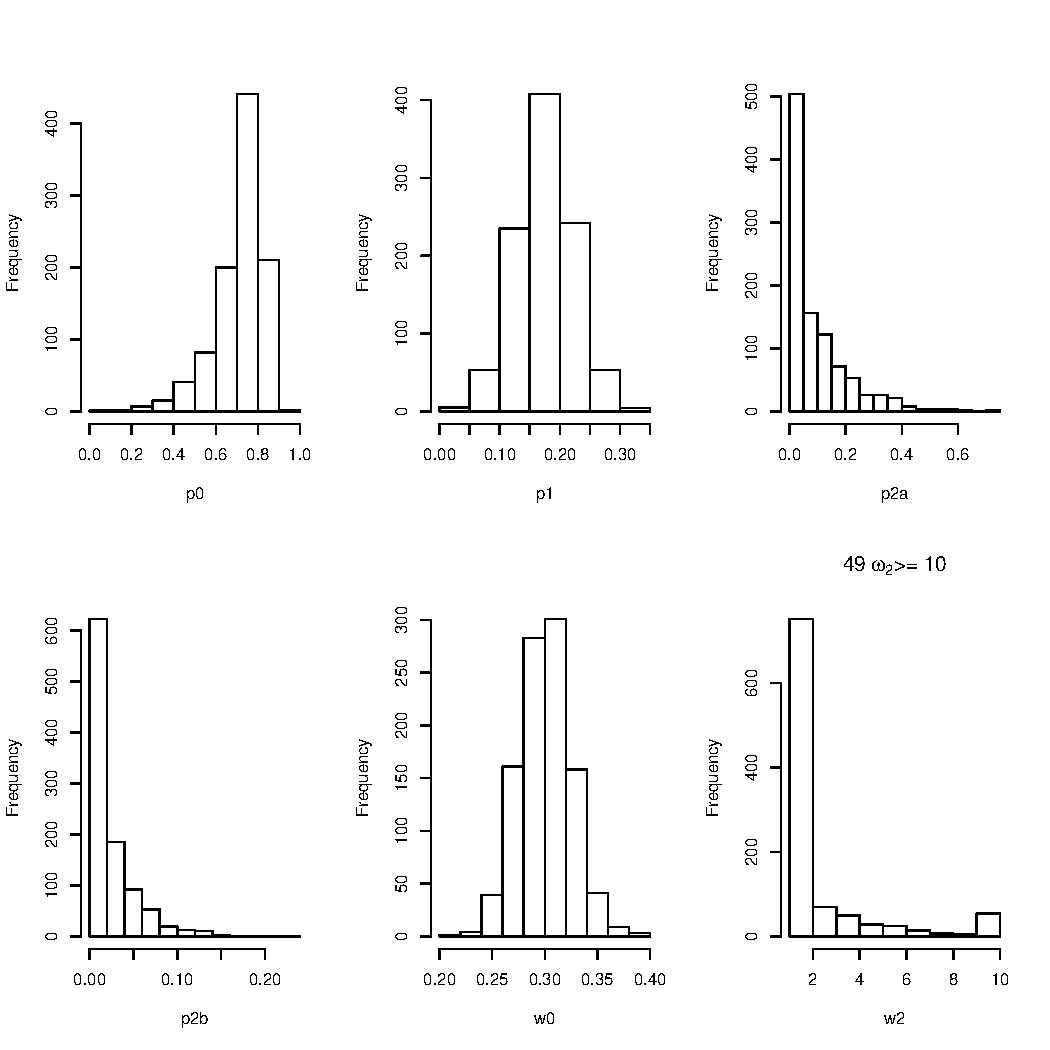
\includegraphics[width=\maxwidth]{figures/data-2} 

}



\end{knitrout}

\clearpage

\begin{lstlisting}
It looks like trouble when p0+p1 is close to 1.

> subset(params,w2>=10)
     p0      p1     p2a     p2b    w0    w2
0.81835 0.17505 0.00544 0.00116 0.28523  23.13062
0.76700 0.22240 0.00822 0.00238 0.30734  93.02138
0.88137 0.11114 0.00665 0.00084 0.31153  14.77213
0.77709 0.21406 0.00693 0.00191 0.25907  10.32459
0.76780 0.22695 0.00405 0.00120 0.31294  30.65330
0.75659 0.24005 0.00255 0.00081 0.26032  72.35850
0.86924 0.12939 0.00119 0.00018 0.34078  13.34368
0.88943 0.10169 0.00796 0.00091 0.35575  31.48847
0.80490 0.18590 0.00748 0.00173 0.30578  14.72235
0.84199 0.14896 0.00769 0.00136 0.31200  26.53156
0.86438 0.13360 0.00175 0.00027 0.34000  11.01535
0.83506 0.15924 0.00478 0.00091 0.31415  27.54533
0.83259 0.15657 0.00912 0.00172 0.32955  11.34695
0.77556 0.20307 0.01693 0.00443 0.34110  10.13749
0.79310 0.19151 0.01240 0.00299 0.26408  11.56291
0.81257 0.18001 0.00608 0.00135 0.29121  32.07342
0.80688 0.18181 0.00923 0.00208 0.30823  13.37337
0.89467 0.09958 0.00517 0.00058 0.34204  11.16014
0.81234 0.17908 0.00703 0.00155 0.31660  48.59562
0.77835 0.21631 0.00418 0.00116 0.31375  63.29933
0.80704 0.17654 0.01348 0.00295 0.30106 998.99714
0.76447 0.22855 0.00537 0.00161 0.27817  33.20885
0.77323 0.19863 0.02239 0.00575 0.37252  15.11797
0.78446 0.20641 0.00723 0.00190 0.34295  32.90619
0.88239 0.11111 0.00577 0.00073 0.33204  10.57666
0.76455 0.23017 0.00406 0.00122 0.32831  21.51810
0.79153 0.20242 0.00482 0.00123 0.25370  49.86961
0.78381 0.20451 0.00926 0.00242 0.30677  14.70206
0.86526 0.12550 0.00807 0.00117 0.32887 112.16901
0.80157 0.19535 0.00247 0.00060 0.28533 318.57920
0.76067 0.22647 0.00991 0.00295 0.28768  24.92604
0.82860 0.16522 0.00515 0.00103 0.30369 998.99975
0.83859 0.15704 0.00368 0.00069 0.30968  32.42859
0.85804 0.13550 0.00557 0.00088 0.30677  37.71321
0.78052 0.20578 0.01084 0.00286 0.33770  16.00260
0.75505 0.23869 0.00476 0.00150 0.31285  11.21459
0.78054 0.21395 0.00432 0.00118 0.29166  23.57525
0.83264 0.16141 0.00498 0.00097 0.31568 482.68724
0.75263 0.24125 0.00463 0.00148 0.31004 998.99984
0.79062 0.20332 0.00482 0.00124 0.29363  16.36648
0.81082 0.17865 0.00863 0.00190 0.29224 998.99977
0.74472 0.24610 0.00691 0.00228 0.26951  65.34070
0.83898 0.14801 0.01106 0.00195 0.33084  38.19227
0.83199 0.15943 0.00720 0.00138 0.29420 102.80490
0.80901 0.18322 0.00634 0.00144 0.35591  23.31654
0.78510 0.20616 0.00693 0.00182 0.33067  89.48316
0.74582 0.24915 0.00377 0.00126 0.28694  50.81805
0.81857 0.16105 0.01702 0.00335 0.30335  12.37413
0.83797 0.14609 0.01358 0.00237 0.32488  12.05585
\end{lstlisting}

\end{document}
